\documentclass[11pt]{article}
\usepackage{amsmath, amssymb}
\usepackage{geometry}
\geometry{margin=1in}
\usepackage{fancyhdr}
\usepackage{lastpage}
\usepackage{parskip} % Better paragraph spacing
\usepackage{titlesec} % Better section formatting
\usepackage{graphicx}
\usepackage{float}
\usepackage[most]{tcolorbox}
\usepackage{lmodern}
\usepackage{caption}
\usepackage{hyperref}

\newtheorem{definition}{Definition}

% Define commands for reusable content
\newcommand{\coursename}{CS-401 Applied Data Analysis}
\newcommand{\lecturenum}{07}
\newcommand{\lecturedate}{\today}
\newcommand{\professor}{Maria Brbic}

\hypersetup{colorlinks=true,linkcolor=blue,urlcolor=blue}

% Configure section spacing
\titlespacing*{\section}{0pt}{2ex plus 1ex minus .2ex}{1.5ex plus .2ex}
% Header / Footer
\pagestyle{fancy}
\fancyhf{}
\fancyhead[L]{\coursename}
\fancyhead[R]{Lecture \lecturenum}
\fancyfoot[L]{EPFL - Computer Science}
\fancyfoot[C]{Author: Jonathan Dutoit}
\fancyfoot[R]{Page \thepage\ of \pageref{LastPage}}

\begin{document}

\begin{center}
  {\large EPFL - Computer Science} \\[0.5em]
  {\Large \textbf{\coursename}} \\[0.5em]
  {\large Lecture \lecturenum\ --- \lecturedate} \\[0.5em]
  {\large Author: Jonathan Dutoit} \\[0.5em]
  {\large Professor: \professor} \\[0.5em]
\end{center}

\vspace{2cm}

\begin{center}
  {\LARGE \textbf{Learning from data: Supervised learning}}
\end{center}

\vspace{1cm}

\textcolor{red}{\textbf{Machine Learning}}

\begin{itemize}
	\item Supervised: We are given input/output pairs (X, y) that are related via a function \textcolor{blue}{y = f(X)}. We would like to "learn" f, and evaluate it on new data. The types are \textcolor{orange}{discrete} \textcolor{blue}{"classification"} and \textcolor{olive}{continuous} \textcolor{blue}{"regression"}
	\item Unsupervised: Given only samples X of the data, we computer a function f such that \textcolor{blue}{y = f(X)} is a "simpler" representation. The types are \textcolor{orange}{discrete} \textcolor{blue}{"clustering"} and \textcolor{olive}{continuous} \textcolor{blue}{"dimensionality reduction"}
\end{itemize}

\section*{Learning goals}

1. k-NN (k nearest neighbors)

2. Tree-based models: decision trees, random forests

3. Logistic regression


\newpage

\begin{center}
  {\LARGE \textbf{K nearest neighbors (k-NN)}
\end{center}
\vspace{0.5cm}

Given a sample, we'd like to find the \textit{k} closest matches in a labelled dataset. The we return the most frequent label among the \textit{k} \\

\noindent
\begin{minipage}[t]{.5\textwidth}
\raggedright

\textcolor{blue}{The data is the model}
\begin{itemize}
	\item No training needed.
	\item Conceptually simple algorithm.
	\item Accuracy generally improves with more data.
	\item Usually need data in memory, but can also be run from disk. \\
\end{itemize}

\textcolor{blue}{Minimal configuration}:
\begin{itemize}
	\item Only one parameter: \textit{k} (number of neighbors)
	\item But two other choices are also important
		\begin{itemize}
			\item Similarity metric
			\item Weighting of neighbors in  voting (e.g., by similarity)
		\end{itemize}
\end{itemize}
\end{minipage}%
\begin{minipage}[t]{.5\textwidth}
\raggetleft
\textcolor{blue}{Classification}
\begin{itemize}
	\item Model is y = f(X), y is from a discrete set (labels)
	\item Given X, compute y = majority vote of the \textit{k} nearest neighbors
	\item Can also use a weighted vote of the neighbors \\
\end{itemize}

\textcolor{blue}{Regression}
\begin{itemize}
	\item Model is y = f(X), y is a real value
	\item Given X, compute y = average value of the \textit{k} nearest neighbors.
	\item Can also use a weighted average of the neighbors.
\end{itemize}
\end{minipage}

\section*{k-NN distance measures}

\begin{itemize}
	\item Euclidean distance: simplest, fast to compute
	\begin{center}
		$d(x, y) = ||x - y||$
	\end{center}
	\item Cosine Distance: good for documents, images, etc.
		\begin{center}
			$d(x, y) = 1 - \frac{x \cdot y}{||x|| \cdot ||y||}$
		\end{center}
	\item Jaccard Distance: for set data:
		\begin{center}
			$d(X, Y) = 1 - \frac{|X \cap Y|}{|X \cup Y|}$
		\end{center}
	\item Hamming Distance: for string data:
	\begin{center}
		$d(x, y) = \sum^{n}_{i = 1}{(x_i \neq y_i)}$
	\end{center}
	\item Manhattan Distance: coordinate-wise distance
	\begin{center}
		$d(x, y) = \sum^{N}_{i=1}{|x_i - y_i|} $
	\end{center}
	\item Edit Distance: for strings, especially genetic data.
\end{itemize}

\section*{Predicting from samples}

Most datasets are \textcolor{blue}{samples} from a (maybe infinite) \textcolor{red}{population}. We are most interest in \textcolor{red}{models of the population}, but we only have access to a \textcolor{blue}{samples}  from the population. 

Hence, we train on a training sample \textcolor{blue}{D} and denote the fitted models as $f_D$. For a new data point (X, y), predictions if $f_D(X)$

Our data-generated model $f_D(X)$ is a  \textcolor{blue}{statistical estimate} of the true function $f(X)$. Because of this, its subject to bias and variance:

 \begin{itemize}
	 \item (Squared) \textcolor{blue}{error} = E[$(f_D(X) -y)^{2}$] (E is expectation over D)
	\item Fact: error can be decomposed into two parts
		\begin{itemize}
			\item \textcolor{blue}{$Error^{2}$} = \textcolor{red}{$Bias^{2}$} + \textit{\textcolor{orange}{Variance}}
			\item \textcolor{red}{Bias} = E[$f_D(X)$ - y] that represents how far off we are on average from the true value. We can overpredict or underpredict. 
			\item \textcolor{orange}{Variance} = $E[(f_D(X) $ - E[f_D(X)])^{2}$] that represents the variance of the estimates.
		\end{itemize}
\end{itemize}

% Quick centered image
\begin{figure}[H]
    \centering
    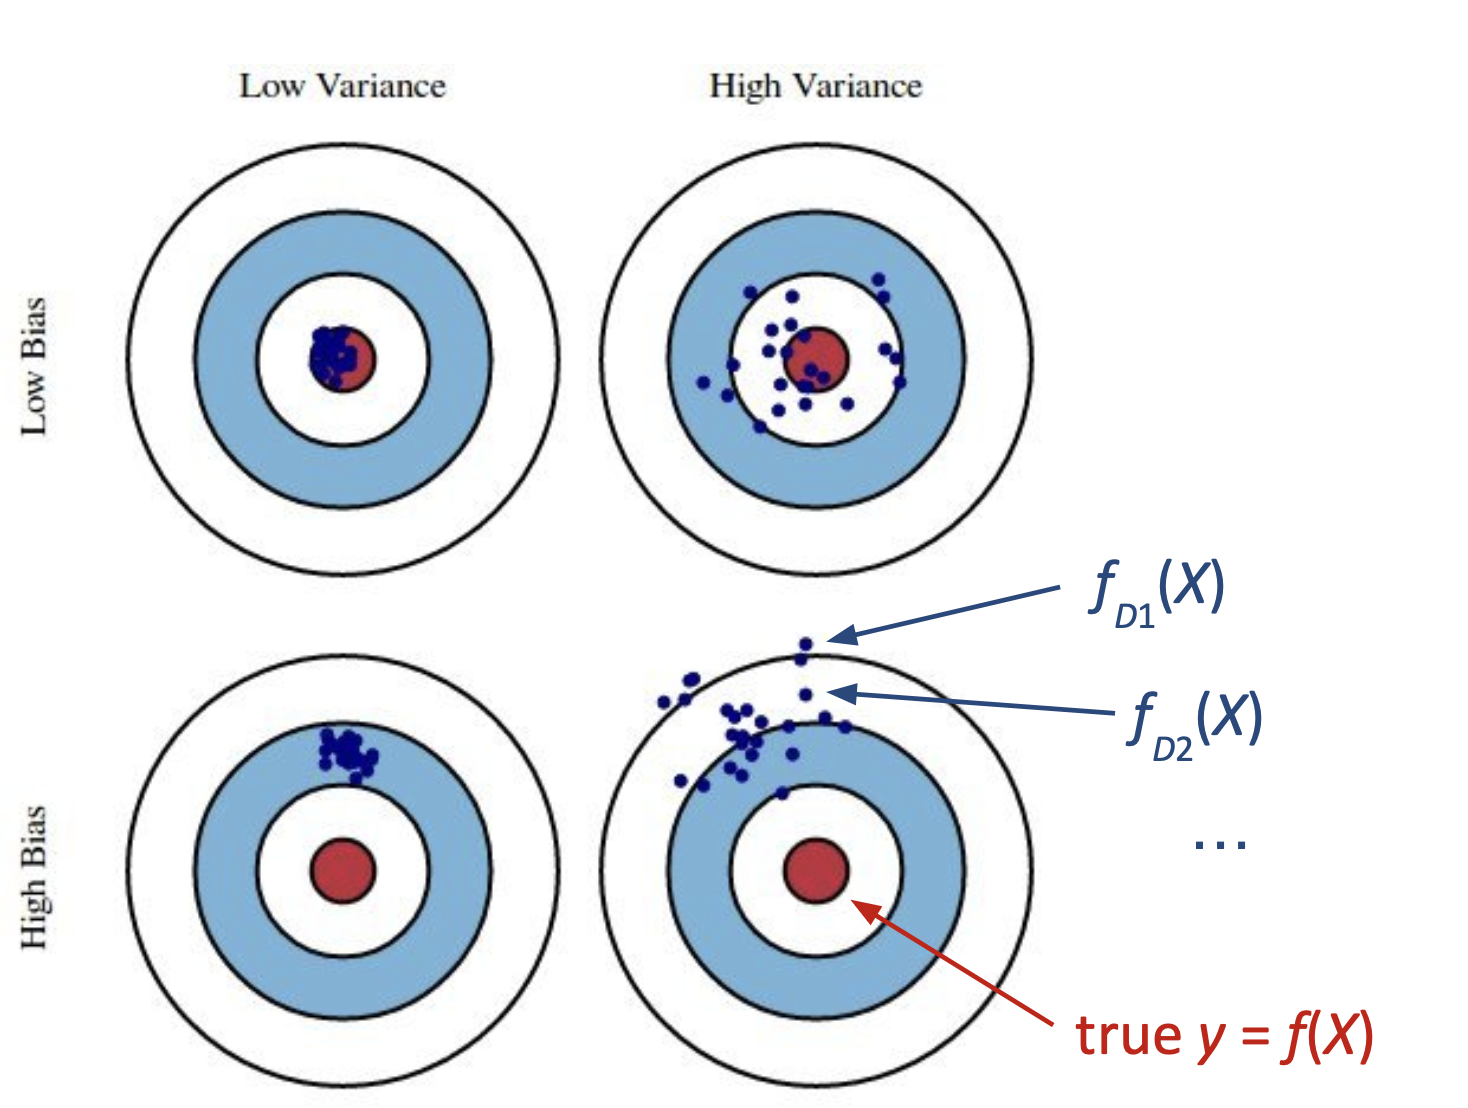
\includegraphics[width=0.7\textwidth]{bias-variance}
    \label{fig:LABEL}
\end{figure}

\section*{Bias/variance tradeoff}

Since $Error^{2} = Bias^{2} + Variance$, there is a tradeoff, usually modulated via model complexity. Hence \textcolor{red}{complex models} (many parameters) usually have lower bias, but higher variance. \textcolor{red}{Simple models} (few parameters) have higher bias, but lover variance. 

\textbf{Example}: a linear model can only fit a straight line. A high-degree polynomial can fit a complex curve. But the polynomial will fit the individual training sample, rather than the full population. Its shape can vary from sample to sample, so it has high variance. 

% Quick centered image
\begin{figure}[H]
    \centering
    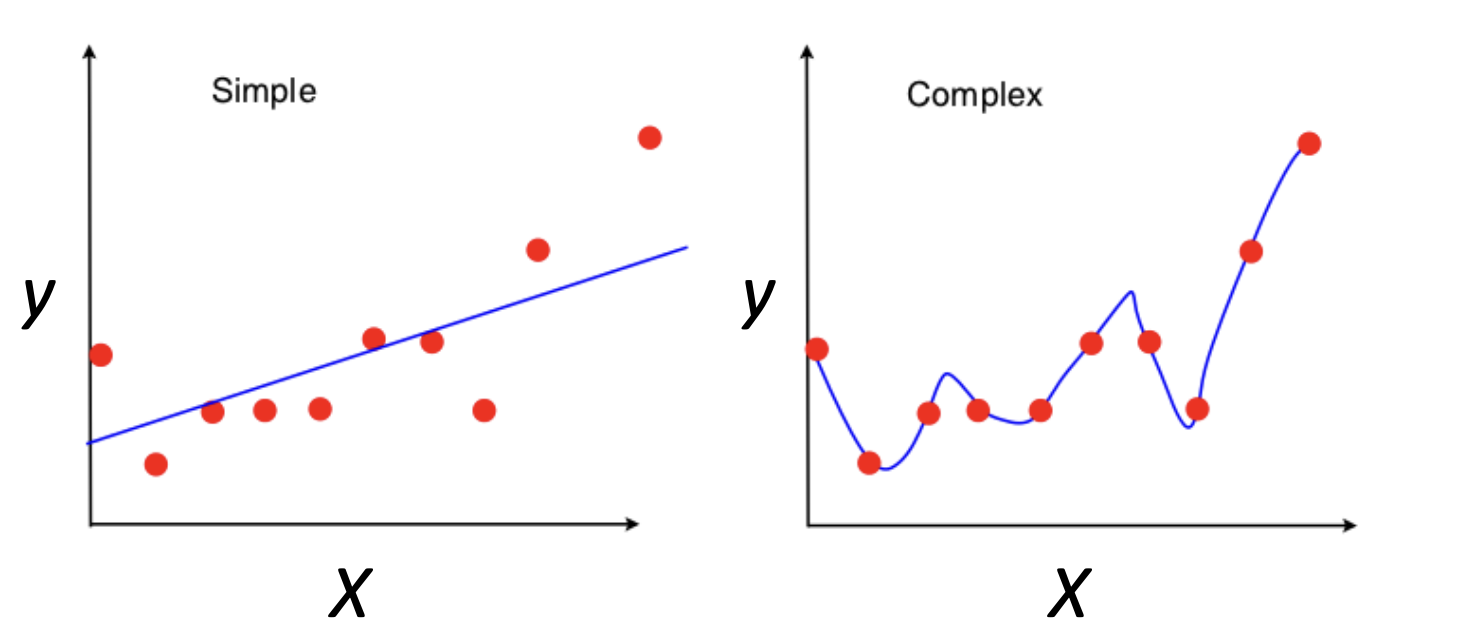
\includegraphics[width=0.8\textwidth]{example-bias-variance}
    \label{fig:LABEL}
\end{figure}

\begin{itemize}
	\item if \textit{variance} strongly dominates, it means there is too much variation between models. This is called \textcolor{red}{over-fitting}
	\item if \textit{bias} strongly dominates, then the models are not fitting the data well enough. This is called \textcolor{red}{under-fitting}
\end{itemize}

\textbf{Choosing k for k nearest neighbors}

\begin{itemize}
	\item Lower \textit{k} $\Rightarrow$ high variance, low bias (if the k is equals to 1, it will always output the predicted value, so no neighbors into account)
	\item Higher \textit{k} $\Rightarrow$ low variance, high bias (if k is the equal to the sample size, then it outputs always the average)
\end{itemize}

\textbf{Choosing \textit{k} in practice}

Use \textcolor{blue}{leave-one-out (LOO) cross-validation}

\begin{itemize}
	\item \textcolor{blue}{Split}: Break data into train and test subsets, e.g., 80-20 \% random split. 
	\item \textcolor{blue}{Predict}: For each point in the training set, predict using the \textit{k} nearest neighbors from the set of all \textit{other} points in training set. Measure the LOO error rate (classification) or squared error (regression). 
	\item \textcolor{blue}{Tune}: Try different values of \textit{k}, and use the one that gives minimum leave-one-out error.
	\item \textcolor{blue}{Evaluate}: Measure error on the test set to quantify performance. 
\end{itemize}

\vspace{0.5cm}

\begin{center}
  {\LARGE \textbf{Decision trees}}
\end{center}
\vspace{0.5cm}

Decision tree learning is a supervised learning approach used in statistics, data mining and machine learning.

In this formalism, a classification or regression decision tree is used as a predictive model to draw conclusions about a set of observations.

Tree models where the target variable can take a discrete set of values are called classification trees; in these tree structures, leaves represent class labels and branches represent conjunctions of features that lead to those class labels.

% Quick centered image
\begin{figure}[H]
    \centering
    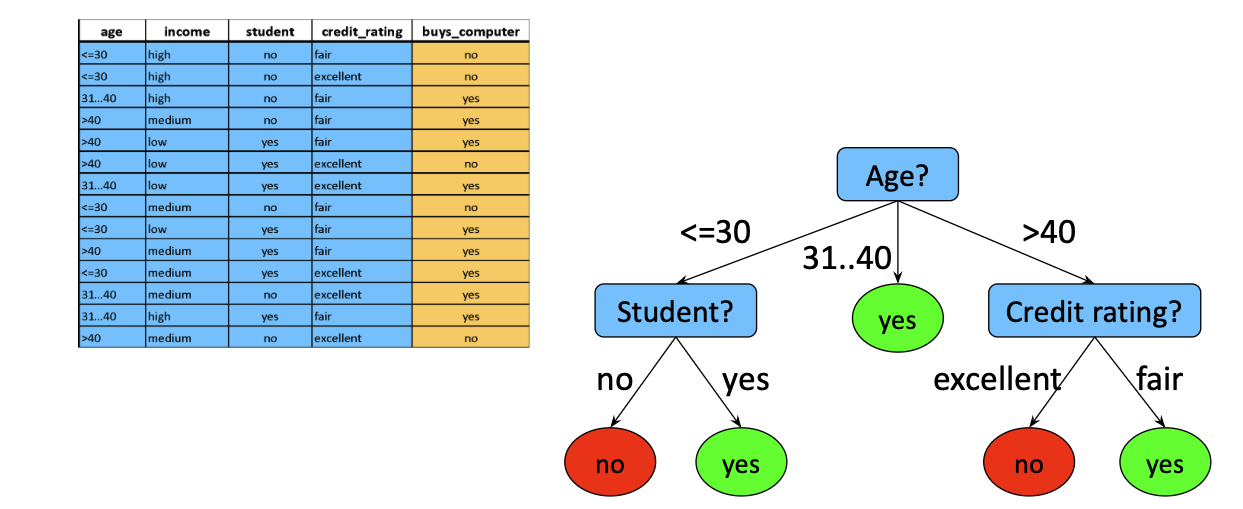
\includegraphics[width=1\textwidth]{decision-trees}
    \label{fig:LABEL}
\end{figure}

\textbf{Goal}: Find decision tree that maximizes classification accuracy on given dataset

\textbf{Optimization}: NP-hard! Heuristic: greedy top-down tree construction + pruning

\begin{tcolorbox}[
  colback=gray!15,     % background color
  colframe=black!50,    % border color
  boxrule=1pt,       % border thickness
  arc=3mm,             % rounded corners
  left=4mm, right=4mm, top=2mm, bottom=2mm % padding
]
\textbf{Formal Definition}

\vspace{0.3cm}

Given a dataset $D = \{(x_i, y_i)\}^{N}_{i=1}$ \\

\begin{itemize}
	\item At each node, the algorithm selects a \textbf{feature j} and a \textbf{threshold t} that best separates the classes (or minimizes prediction error in regression) \\
\end{itemize}

We define impurity (for classification) using metrics like: \\

\begin{itemize}
	\item Entropy
	\[
		H(D) = - \sum^{K}_{k=1}p_k\log_{2}(p_k)
	.\] 
\end{itemize}
\\
For regression: 

\[
	MSE(D, j, t) = \frac{1}{|D_L|} \sum_{i \in D_L} (y_i - \hat{y_L})^{2} + \frac{1}{|D_R|} \sum_{i \in D_R} (y_i - \hat{y_R})^{2}
.\] 

\\ 

and we choose the split minimizing MSE.
\end{tcolorbox}

\textbf{Tree Growth and Stopping}

\begin{itemize}
	\item \textbf{Recursive Binary Splitting}: Split nodes greedily until a stopping condition:
		\begin{itemize}
			\item Max depth
			\item Min samples per leaf
			\item Min impurity decrease
\end{itemize}
		
	\item \textbf{Pruning}: To prevent overfitting, prune the tree using:
		\begin{itemize}
			\item Cost Complexity Pruning (CART): minimize
			\[
				C_{\alpha}(T) = R(T) + \alpha|T|
			.\] 
			Where $R(T)$ is misclassification cost and $|T|$ is number of leaves. 
		\end{itemize}
\end{itemize}

\textbf{Advantages and Disadvantages}

\begin{minipage}[T]{0.5\textwidth}

\textbf{Pros}:
\begin{itemize}
	\item Easy to interpret and visualize
	\item Handles numerical and categorical features
	\item Requires little data preprocessing (no scaling, normalization)
\end{itemize}
\end{minipage}
\begin{minipage}[T]{0.5\textwidth}

\textbf{Cons}:
\begin{itemize}
	\item High variance (overfits easily)
	\item Small changes in data can change the tree structure drastically
	\item Greddy nature means not globally optimal.
\end{itemize}
\end{minipage}

\section*{Ensemble methods}

Are, metaphorically, like \textcolor{red}{"democratic" machine learning algorithms}:
\begin{itemize}
	\item Take a collection of simple or \textit{weak} learners
	\item Combine their results to make a single, better learner
\end{itemize}
\textbf{Types}:
\begin{itemize}
	\item \textcolor{red}{Bagging}: train learners in parallel on different samples of the data, then combine by voting (for discrete output) or by averaging (for continuous output)
	\item \textcolor{red}{Boosting}: train learner again, but after filtering/weighting samples based on output of previous train/test runs
	\item \textcolor{red}{Stacking:} combine outputs from various models using a second-stage learner (e.g., linear regression).
\end{itemize}

\section*{Random forests}

Grow \textit{K} trees on datasets \textcolor{red}{sampled} from the original dataset (size N) with replacement (bootstrap samples), \textit{p} = number of features. 

\textcolor{purple}{\textbf{Principles:}} we want to take a \textcolor{red}{vote between different learners} so we don't want the models to be too similar. The following two criteria (\textcolor{blue}{blue comments}) ensure \textcolor{red}{diversity} in the individual trees:

\begin{itemize}
	\item Draw \textit{K} bootstrap samples of size \textit{N}.
		\begin{itemize}
			\item \textcolor{blue}{Each tree is trained on different data.}
		\end{itemize}
	\item Grow each decision tree by selecting a \textcolor{red}{random set of \textit{m} out of \textit{p} features} at each node and choosing the best feature to split on.
		\begin{itemize}
			\item \textcolor{blue}{Corresponding nodes in different trees (usually) can't use the same feature to split on.}
		\end{itemize}
	\item At testing time, aggregate the predictions of the trees (most popular vote, or average) to produce the final class (example of bagging).
\end{itemize}

Typically \textit{m} might be e.g., \verb|sqrt(p)|, but can be smaller. 

\begin{itemize}
	\item \textcolor{lime}{Very popular in practice}, probably the most popular classifier for dense data (up to a few thousand features)
	\item \textcolor{lime}{Easy to implement} (simply train many normal decision trees)
	\item \textcolor{lime}{Easy to parallelize}
\end{itemize}

\begin{itemize}
	\item \textcolor{red}{Needs many passes over the data} - at least the max depth of the trees
\end{itemize}

\section*{Boosted decision trees}

A more recent alternative to random forests. In contrast to RF, whose trees are trained \textcolor{red}{independently} by bagging, BDT trees are trained \textbf{\textcolor{red}{sequentially}} by \textbf{\textcolor{red}{boosting}}: Each tree is trained to predict ("correct") residual errors of previous trees ($\Rightarrow$ bias reduction).

\textbf{Final prediction}: sum of predictions made by individual trees. 

\begin{itemize}
	\item Both RF and BDT can produce very high-quality models. Superiority of one method or the other is dataset-dependent. 
	\item Resource requirements are very different as well, so it's actually non-trivial to compare the methods.
	\item The "geometry" of the methods is very different. For instance, RF use 10's of deep, large trees. Bias reductions comes through depth and variance reduction through the ensemble aggregate. Boosted decision trees use 1000's of shallow, small trees. Bias reduction through boosting, variance is already low. 
\end{itemize}

\vspace{0.5cm}

\begin{center}
  {\LARGE \textbf{Logistic regression}}
\end{center}
\vspace{0.5cm}

In statistic, a \textbf{logistic model} is a statistical model that models the \textbf{log-odds} of an event as a \textbf{linear combination} of one or more independent variables. Hence, in regression analysis, logistic regression estimates the parameters of a logistic model. 

It's a supervised machine learning algorithm widely used for \textbf{binary classification tasks}. This approach utilizes the logistic (or sigmoid) function to transform linear combination of input features into a probability value ranging between 0 and 1. 

This probability indicates the \textbf{likelihood} that a given input corresponds to one of two predefined categories. 

% Quick centered image
\begin{figure}[H]
    \centering
    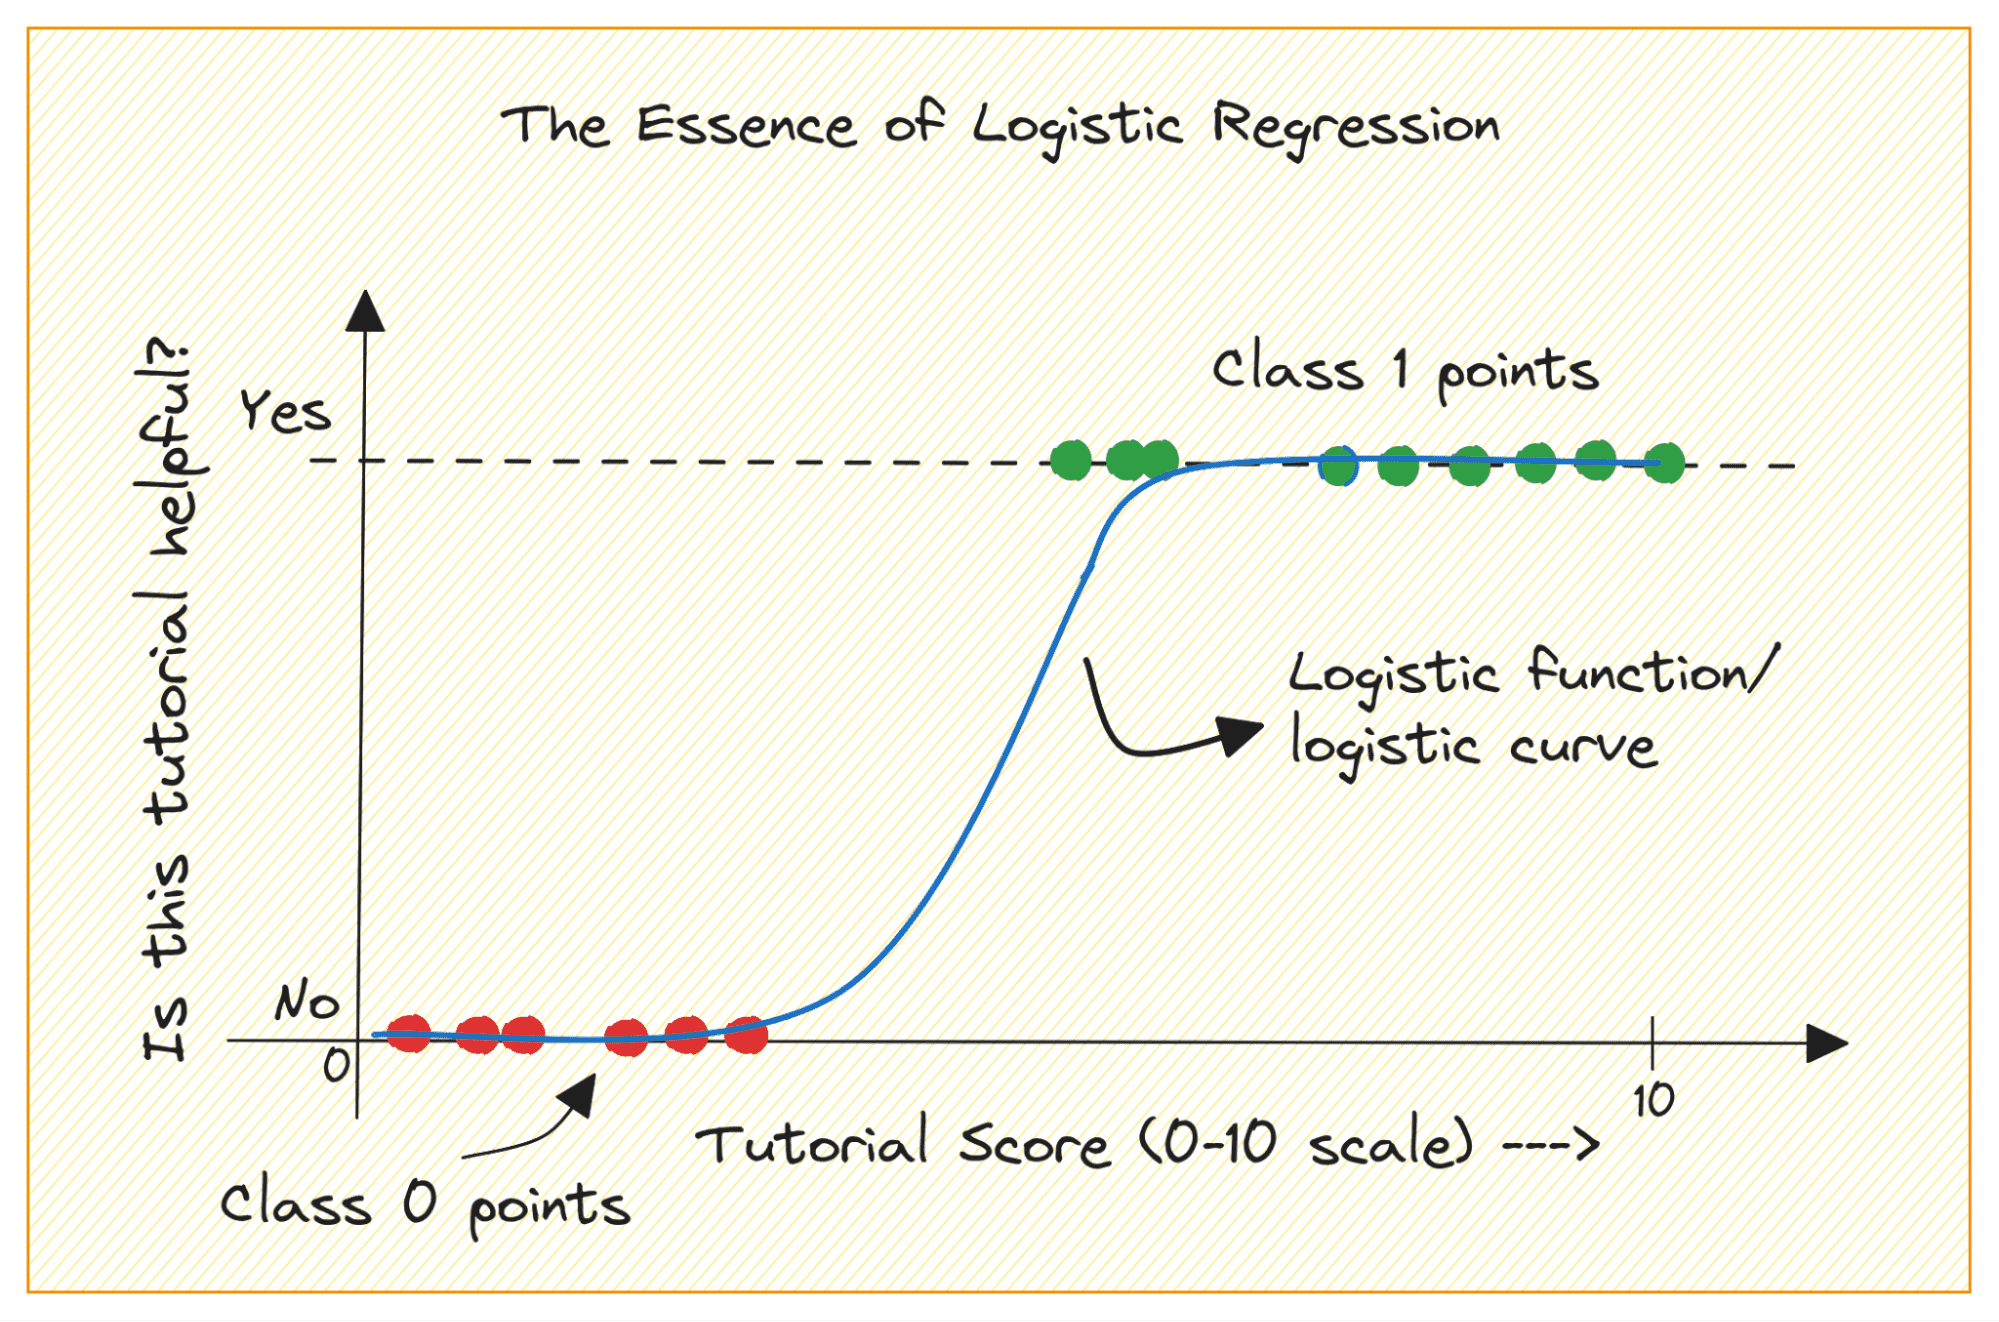
\includegraphics[width=0.5\textwidth]{logistic-regression}
    \label{fig:LABEL}
\end{figure}

With its distinctive S-shaped curve, the logistic function effectively maps any real-valued number to a value within the 0 to 1 interval. This feature renders it particularly suitable for binary classification tasks. 
The logistic (sigmoid) function is of the form: 
\[
	p(x) = \frac{1}{1 + e^{-(x - \mu)/s}}
.\]

where $\mu$ is a location parameter (the midpoint of the curve, where $p(\mu) = 1/2$ and \textit{s} is a scale parameter. This expression may be rewritten as: 
\[
	p(x) = \frac{1}{1 + e^{-(\beta_0 + \beta_1 x)}}
.\] 

where $\beta_0 = - \mu/s$ and is known as the intercept (it is the vertical intercept or y-intercept of the line $y = \beta_0 + \beta_1 x$), and $\beta_1 = 1/s$ (inverse scale parameter or rate parameter): these are the \textit{y}-intercept and slope of the log-odds as a function of x.

\textbf{Optimization}: finding best model via maximum likelihood. 
\begin{itemize}
	\item Don't use square loss as in linear regression (where \textit{y} is assumed to be generated from Normal distribution)
	\item Use cross-entropy loss instead (\textit{y} assumed to be generated from Bernoulli distribution, i.e., biased coin)
\end{itemize}

The more features the better? \textcolor{red}{No!}. More features mean less bias, but more variance, which implies overhitting. 

Carefully selected features can improve model accuracy. 
\begin{itemize}
	\item E.g, keep features that correlate with the label \textit{y}
	\item Forward/backward feature selection
	\item Regularization (e.g., penalize norm of weight vector)
\end{itemize}

\end{document}
